\chapter{Einführung in die Qualitätssicherung}
\label{cha:einfuehrungQS}

    Um das Ziel der Qualitätssicherung zu verstehen, wird die Qualitätssicherung zunächst vom Qualitätsmanagement abgegrenzt. Das Qualitätsmanagement stellt alle Maßnahmen zur Führung und Steuerung der Qualität im Unternehmen dar, während die Qualitätssicherung \enquote{als Bestandteil des Qualitätsmanagements alle organisatorischen und technischen Maßnahmen, die vorbereitend, begleitend und prüfend der Schaffung und Erhaltung einer definierten Qualität eines Produkts oder einer Dienstleistung dienen.}\footnote{Springer (Qualitätssicherung).} Dabei geht es nicht darum, ein Produkt kontinuierlich zu verbessern, sondern ein vorgegebenes Niveau zu erreichen oder zu halten.

    \begin{quote}
        \enquote{Die Darlegung des Qualitätsmanagements, d.h. alle Tätigkeiten zur Schaffung von Vertrauen, dass die Qualitätsanforderungen erfüllt werden, wird Qualitätssicherung genannt. Als zentrale Maßnahmen braucht es regelmäßige Überprüfungen, ob das Qualitätsmanagementsystem wie geplant funktionert und ob die vorgesehenen Qualitätsmaßnahmen wirklich durchgeführt werden. Solche Überprüfungen heißen Audits.}\footnote{Glinz (Software Engineering), S.120.}
    \end{quote}

    Im Projekt unterscheidet man außerdem zwischen organisatorischen, analytischen und konstruktiven Maßnahmen zur Sicherung der Qualität. Diese werden im Folgenden definiert:

    \begin{description}
        \item[Organisatorische Maßnahmen] Definiert die Aufbau- und Ablauforganisation , die die Softwarequalität im Projekt verankert. Dies schafft die Voraussetzung dafür, dass analytische und konstruktive Maßnahmen durchführbar und wirksam sind.\footnote{Vgl. Schneider (Abenteuer Softwarequalität), S.177.}
        \item[Analytische Qualitätssicherung] In analytischen Verfahren wird ein bereits fertiger Prüfling untersucht, um Fehler zu finden. Analytische Maßnahmen wirken sich auf die Softwarequalität indirekt aus, wenn nämlich die gefundenen Fehler beseitigt werden. Die analytische Qualitätssicherung umfasst das Testen der Software.\footnote{Vgl. Schneider (Abenteuer Softwarequalität), S.177.}
        \item[Konstruktive Qualitätssicherung] Maßnahmen, die bereits bei der Konstruktion von Software auf die Verbesserung ausgewählter Qualitätsaspekte abzielen und nicht erst nachträglich durch Prüfung und Korrektur. Konstruktive Maßnahmen können daher häufig verwendete Standards und Rahmenwerke sein. Darunter fallen auch Qualitätsmanagementsysteme und -modelle wie die ISO 9000 oder Six Sigma.\footnote{Vgl. Schneider (Abenteuer Softwarequalität), S.177.}
    \end{description}

%----------------------------------
%
% Organisatorische Qualitätssicherungsmaßnahmen
%
%----------------------------------
    \section{Organisatorische Qualitätssicherungsmaßnahmen}

        Qualität im Projekt muss an drei Stellen umgesetzt werden und zwar in der Aufbauorganisation, der Ablauforganisation und in Form eines Qualitätsmanagementsystems.

        \subsection{Aufbauorganisation}

            Die Aufbauorganisation bezieht sich dabei auf die Ansiedlung der Qualitätssicherung im Organisationsdiagramm des Unternehmens. Bei einer klassischen, hierarchieschen Struktur ist es zwingend erforderlich, dass die Qualitätsbeauftragten auf allen Hierarchieebenen vertreten sind, ohne, dass die normalen Projektteilnehmer eine Weisungsbefugnis gegenüber diesen haben.\footnote{Vgl. Schneider (Abenteuer Softwarequalität), S.12f.}

            \begin{figure}[!htbp]
                \begin{center}
                    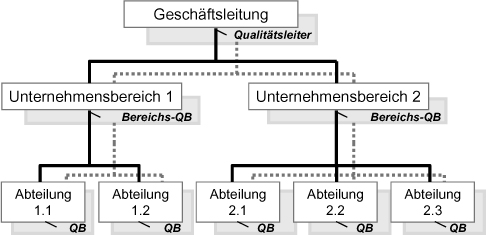
\includegraphics[width=11cm]{Abbildungen/aufbauqs}
                    \caption[Aufbauorganisation mit Qualitätsbeauftragten]{Aufbauorganisation mit Qualitätsbeauftragten\protect\footnotemark}
                    \label{abb:aufbauqs}
                \end{center}
            \end{figure}

            \footnotetext{Schneider (Abenteuer Softwarequalität), S.13.}

            \autoref{abb:aufbauqs} stellt die Soll-Hierarchie in einem Unternehmen dar, dass die Qualitätssicherung in den Fokus stellt. Die \emph{Qualitätsbeauftragten} (QB) sind jeweils auf einer Hierarchiebene mit den Leitern ihrer jeweiligen Abteilungen und empfangen weder von ihren Kollegen, noch von deren Vorgesetzten Weisungen. Sie sind nur gegenüber höher gestellten Qualitätsbeauftragten rechenschaftspflichtig.\footnote{Vgl. Schneider (Abenteuer Softwarequalität), S.13f.}

            Das Qualitätsteam bekommt \enquote{Narrenfreiheit}, was ihnen erlaubt offen Kritik zu üben, ohne Konsequenzen fürchten zu müssen. Diese sollte allerdings gerechtfertigt sein, sodass die negative Konnotation, dass die Narrenfreiheit \enquote{Dümmlichkeit} impliziert, entfällt.\footnote{Expertengespräch mit R. Bihler, SAP SE.}

            Mit Hilfe dieser Struktur wird verhindert, dass Qualitätsverantwortliche durch Druck ihrer Vorgesetzten die eigenen Ansprüche herunterschrauben, da ansonsten Deadlines oder Budgetziele des Projekts nicht haltbar wären.\footnote{Vgl. Schneider (Abenteuer Softwarequalität), S.13.}

        \subsection{Ablauforganisation}

            \begin{quote}
                \enquote{Innerhalb der Ablauforganisation muss das Qualitätsmanagementsystem für alle Abläufe die qualitätsrelevanten Kompetenzen, Verantwortlichkeiten und gegenseitigen Beziehungen festlegen. Man ist dabei bestrebt, möglichst wenig Qualitätsaufgaben separat zu regeln, sondern diese weitestgehend in die Prozesse des Unternehmens zu integrieren.}\footnote{Glinz (Software Engineering), S.119.}
            \end{quote}

            \begin{figure}[!htbp]
                \begin{center}
                    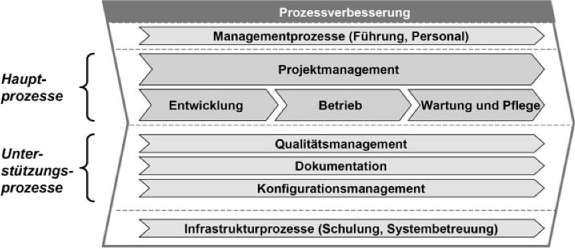
\includegraphics[width=11cm]{Abbildungen/ablaufqs}
                    \caption[Qualitätsmanagement als Unterstützungsprozess]{Qualitätsmanagement als Unterstützungsprozess\protect\footnotemark}
                    \label{abb:ablaufqs}
                \end{center}
            \end{figure}

            \footnotetext{Schneider (Abenteuer Softwarequalität), S.14.}

            \autoref{abb:ablaufqs} zeigt, dass der Qualitätsprozess nicht einsam und für sich stehen soll, sondern eine enge Verwebung mit den bestehenden Prozessen des Unternehmens angestrebt wird. Die Qualitätsprozesse sind unterstützend zum Entwicklungsprozess der Software, da mit qualitativer Software und nicht mit qualitativen Softwareentstehungsprozessen Geld verdient werden kann. Der Qualitätsprozess dient somit zur Unterstützung der Projektprozesse.

        \subsection{Qualitätsmanagementsystem}

            Das Qualitätsmanagementsystem sind nach ISO 8402 alle
            \begin{quote}
                zur Verwirklichung des Qualitätsmanagements erfoderliche Organisationsstruktur, Verfahren, Prozesse und Mittel.\footnote{Schneider (Abenteuer Softwarequalität), S.15.}
            \end{quote}
            Dies steht in direkter Verbindung mit der ISO 8402 Definition des Qualitätsmanagements:
            \begin{quote}
                Alle Tätigkeiten der Gesamtführungsaufgabe, welche die Qualitätspolitik, Ziele und Verantwortlichkeiten festlegen sowie diese durch Mittel wie Qualitätsplanung, -lenkung, -sicherung und -verbesserung im Rahmen des Qualitätsmanagementsystems verwirklichen.\footnote{Schneider (Abenteuer Softwarequalität), S.15.}
            \end{quote}

            Zusammenfassend ist Ziel des Qualitätsmanagementsystems eine Verbesserung des gesamten Unternehmens auf der Prozess bzw. Produktebene. Auf Software angewandt bedeutet dies, dass das Qualitätsmanagementsystem sicherstellt, dass die Software alle internen und externen Ansprüche erfüllt. Dabei ist Qualität kein Selbstzweck, sondern dient stets der Verbesserung des Produkts.

%----------------------------------
%
% Analytische Qualitätssicherungsmaßnahmen
%
%----------------------------------
    \section{Analytische Qualitätssischerungsmaßnahmen}
    \label{subsec:analytischeqs}

        Analytische Qualitätssicherungsmaßnahmen beziehen sich auf Schritte, die nach der Entwicklung einer Software darauf abzielen, die korrekte Funktion eben dieser sicherzustellen. Das bedeutet insbesondere, dass neben einer aktuellen Dokumentation eine Menge von Tests durchgeführt werden müssen, die überprüfen, ob die Software auf Eingaben mit den erwarteten Ausgaben reagiert. Die Länge der Testphase, die sich an die Entwicklung anschließt, kann oft nicht korrekt festgelegt werden, da nicht abzusehen ist, wie viel Code korrigiert werden muss und wie schwerwiegend die Fehler sind. Somit gefährdet die Testphase meist die vorher festgelegte Projektlaufzeit und das Projektbudget.\footnote{Schneider (Abenteuer Softwarequalität), S.83ff.}

        Obwohl die Testphase häufig unerwünscht ist, ist sie essentiell, da Fehler, die noch während des Projekts entdeckt werden, günstiger zu beheben sind, als im späteren Verlauf. Je nach Einsatzgebiet der Software kann ein Fehler der Software die Kosten des Testvorgangs weit übersteigen. Aufgrund dessen sollte jedes Teilprodukt einer Software so früh wie möglich geprüft werden.\footnote{Prechelt (Vorlesung Softwaretechnik), S.6.}

        Ein Test ist nach IEEE Standard 610.12 definiert als:
        \begin{itemize}
            \item \enquote{The process of operating a system or component under specified conditions, observing or recording the results, and making an evaluation of some aspect of the system or component.}
            \item \enquote{The process of analyzing a software item to detect the differences between existing and required conditions (that is, bugs) and to evaluate the features of the software items.}\footnote{IEEE 610.12 (Standard Glossary), S.20.}
        \end{itemize}

        Testen ist daher die Anwendung der Software mit dem Ziel diese zum Absturz oder zu einer falschen Ausgabe zu führen, um diese Fehler zu dokumentieren. Um möglichst viele Fehler und Probleme abzudecken existiert eine große Menge an Testverfahren. Diese werden in dynamische Verfahren und statische Verfahren unterteilt. Die dynamischen Verfahren haben gemein, dass die Software im Rahmen des Tests ausgeführt wird und mit verschiedenen Parametern und auf verschiedenen Laufzeitumgebungen ausgeführt wird. Bei statischen Testverfahren wird der Programmcode geprüft, ohne, dass dieser ausgeführt wird. Bei der statischen Analyse wird die Einhaltung von Standards geprüft und es werden Statistiken zum Quellcode erstellt, die beispielsweise Verzweigungen und die Codezeilenanzahl dokumentieren. Dynamische Tests prüfen dagegen eine Vielzahl von Anwendereingaben und Parametern, um mögliche Fehler zu finden. Nachfolgend sind dynamische und statische Testverfahren beispielhaft gelistet. Als Beispiel für einen statischen Test dient der Strukturtest und für dynamische Tests der Funktionstest.\footnote{Vgl. Prechelt (Vorlesung Softwaretechnik), S.10f.}

        \subsection{Strukturtest}

            Ein Strukturtest, auch \emph{White Box/Glass Box Test} genannt, betrachtet Testfälle auf Grundlage der Implementation einer Komponente.
            Dies bedeutet, dass nicht nur eine klassische Funktion aus Anwenderperspektive gestartet wird, sondern dass die Bestandteile des Codings überprüft werden. Die geschieht auf bis zu vier Ebenen:
            \begin{itemize}
                \item Anweisungsüberdeckung ($C_0$)
                \begin{itemize}
                    \item Jede Anweisung muss mindestens einmal ausgeführt werden
                    \item Ist für Fehlerbehandlungscode meist schwierig oder sogar unmöglich
                \end{itemize}
                \item Bedingungsüberdeckung ($C_1$)
                \begin{itemize}
                    \item Zusätzlich: Jede Steuerbedingung (bei if, while, switch etc.) war mindestens einmal falsch und einmal wahr
                \end{itemize}
                \item Schleifenüberdeckung ($C_2$)
                \begin{itemize}
                    \item Zusätzlich: Jede Schleife wird einmal 0-fach, einmal 1-fach und einmal mehrfach durchlaufen
                \end{itemize}
                \item Datenflusskriterien
                \begin{itemize}
                    \item Mehrere Kriterien, die beispielsweise bei gesetzten Variable auch eine Verwendung fordern.\footnote{Vgl. Prechelt (Vorlesung Softwaretechnik), S.22.}
                \end{itemize}
                \end{itemize}

        \subsection{Funktionstest}

            Das Pendant zum Strukturtest stellt der Funktionstest dar. Dieser wird auch \emph{Black Box Text} genannt, da nur Ein- und Ausgaben betrachtet werden. Wie die Eingaben im Programm verarbeitet werden, wird im Strukturtest geprüft.

            Die Herausforderung des Funktionstests ist es, vorab das erwartete Resultat festzulegen, das bei einer Buchhaltungssoftware sehr kompliziert und umständlich zu errechnen ist. Im besten Fall werden die erwarteten Resultate schon vor der Implementierung festgelegt, um eine Referenz zur Funktionsfähigkeit des Programms festzulegen. Dies wird beispielsweise bei Unit-Tests angewandt, die eine kleine Teilkomponente eines Programms ausführen und mit einem gewünschten Ergebnis gegenprüfen.\footnote{Vgl. Prechelt (Vorlesung Softwaretechnik), S.13ff.}

%----------------------------------
%
% Konstruktive Qualitätssicherungsmaßnahmen
%
%----------------------------------
    \section{Konstruktive Qualitätssicherungsmaßnahmen}

         \begin{quote}
                \enquote{Eine Technik, eine Maßnahme, ein Teilprodukt oder ein Prozess werden konstruktiv zur Qualitätsverbesserung eingesetzt, weil man aus Erfahrung weiß, dass sie sich dafür schon bewährt haben, und wo das gelungen ist.}\footnote{Schneider (Abenteuer Softwarequalität), S.179.}
            \end{quote}

            Demnach ist es nicht nur das Ziel von konstruktiven Maßnahmen Fehler zu entdecken und nachträglich auszubessern, sondern die Entstehung von Fehlern schon frühzeitig zu verhindern. Dies kann durch anerkannte Normen, Best-Practices aus alten Projekten oder durch Erfahrung im Umgang mit Projekten erreicht werden. Außerdem sollten erkannte Fehler im Produkt nicht bloß ausgebessert, sondern auch die Ursache des Fehlers aufgedeckt und behoben werden.\footnote{Vgl. Schneider (Abenteuer Softwarequalität), S.179f.}

%----------------------------------
%
% Ausgewählte Methoden der Qualitätssicherung
%
%----------------------------------
    \section{Ausgewählte Methoden der Qualitätssicherung}
    \label{sec:qsmethoden}

        \subsection{ISO 9000}
        \label{subsec:iso9000}

            Die ISO 9000 ist untergliedert in vier Unternormen, die ISO 9001 bis 9004. Die ISO 9001 umfasst dabei ISO 9002 und ISO 9003 und dient als Zertifizierungsnorm für Qualitätsmanagementsysteme.\footnote{Vgl. Carlsen (ISO-9000), S.10.}

            Die ISO 9001 gibt keine konkreten Werkzeuge und Methoden vor, um Qualität zu erreichen, sondern erklärt nur wofür Modelle vorgelegt werden müssen und was zu dokumentieren ist. Anhand dieser Standards kann das vorhandene Qualitätsmanagement eines Unternehmens bewertet und zertifiziert werden.

            Nachfolgend werden die Schritte dargestellt, die nötig sind um nach der ISO 9001 zertifiziert zu werden. Dies bedeutet, dass im Unternehmen ein Qualitätsmanagementsystem besteht, dokumentiert ist und angewendet wird.

            Die ISO 9001 setzt vier Elemente voraus, die im Unternehmen gegeben sein sollen:
            \begin{itemize}
              \item \enquote{Sie definiert, dass es Menschen im Unternehmen geben muss, die sich des Themas Qualität annehmen.
              \item Sie legt fest, dass Verfahren im Unternehmen festgelegt und implementiert sein müssen.
              \item Sie nennt einige Verfahren, die immer vorhanden sein müssen.
              \item Sie bestimmt, wie die Wirksamkeit des QM-Systems und seiner Prozesse überwacht und überprüft werden muss.}\footnote{Pfitzinger (ISO 9000 zu TQM), S.13.}
            \end{itemize}

            Wenn die zuvor vorgestellten organisatorischen Maßnahmen umgesetzt wurden und Qualitätsbeauftragte auf jeder Ebene des Unternehmens etabliert wurden, ist die erste Bedingung, die Anwensenheit von qualitätssichernden Mitarbeitern gegeben. Die Hierarchie und die Aufgabe der zuständigen Mitarbeiter sollte zusätzlich dokumentiert werden, um einen Nachweis zur Qualität zu liefern.

            Die Verfahren, die im Unternehmen stattfinden, sollten umfassend dokumentiert sein. Insbesondere die Interaktionen mit Kunden und Lieferanten und sonstigen Externen muss schriftlich vorliegen, um von Seiten des Unternehmens unabhängig von den ausführenden Personen kontinierliche Leistungen zu erbringen.\footnote{Vgl. Pfitzinger (ISO 9000 zu TQM), S.14.} Die Pflichtverfahren umfassen:
            \begin{itemize}
              \item Lenkung von Dokumenten
              \item Lenkung von Aufzeichnungen
              \item Internes Audit
              \item Lenkung fehlerhafter Produkte
              \item Korrekturmaßnahmen
              \item Vorbeugungsmaßnahmen\footnote{Thode (Pflichtverfahren ISO 9001).}
            \end{itemize}
            Für diese muss ein dokumentierter Prozess vorliegen.

            Zuletzt muss das Qualitätsmanagementsystem vom Unternehmen auf seine Wirksamkeit geprüft werden, damit die Zertifizierung nicht als einzige Kontrolle dient. Hierzu dienen interne Audits, die das System überprüfen und beispielsweise jährlich testen, ob es zertifiziert werden könnte. Außerdem sollen die Qualitätsbeauftragten auf den hohen Hierarchieebenen in regelmäßigen Abständen eine Bewertung zum Stand der Qualität im Unternehmen abgeben.\footnote{Vgl. Pfitzinger (ISO 9000 zu TQM), S.15.}

            Die ISO 9001 gibt zudem den Deming-Zyklus als Modell vor. Dieser sieht vier Schritte vor, die iterativ durchlaufen werden, um optimale Qualität zu gewährleisten.\footnote{Vgl. Dahl (Gebrauchsanleitung ISO 9001).}
            \begin{figure}[H]
                \begin{center}
                    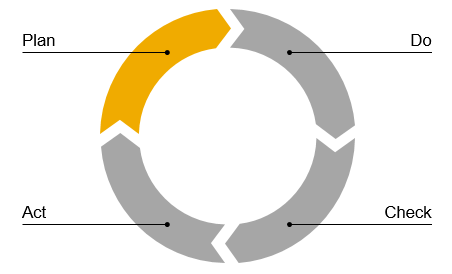
\includegraphics[width=9cm]{Abbildungen/pdca}
                    \caption{Deming-Zyklus}
                    \label{abb:pdca}
                \end{center}
            \end{figure}

            Der Zyklus wird in \autoref{abb:pdca} dargestellt. Der Startpunkt ist in Gold hervorgehoben und der Zyklus beginnt mit der Planung, wie der Prozess bzw. das Endprodukt, die Software, aussehen soll um danach die geplanten Prozesse zu durchlaufen. Am Ende dieser Durchläufe folgt die Prüfungsphase in der mit statistischen Methoden kontrolliert wird, ob die in der Planungsphase gesteckten Anforderungen erfüllt wurden. Auf Grundlage dieser Ergebnisse werden Maßnahmen beschlossen, um die Prozesse und Produkte zu optimieren und somit einen kontinuierlichen Verbesserungsprozess im Unternehmen zu etablieren.

            \subsubsection{Total Quality Management}

            \begin{quote}
              \enquote{TQM [Total Quality Management; Anm. d. Autors] is [seen] as a continuois process of improvement for individuals, groups of people and whole organisations.}\footnote{Kanji (Make ISO 9000 more effective), S.67.}
            \end{quote}

            Total Quality Management ist ein umfassendes Managementkonzept, dass die Grundlage für viele heute existierende Qualitätsmanagementsmodelle bildet. Es betrachtet neben den Anforderungen der Kunden und Mitarbeiter an die Qualität der Software, die Belange aller Stakeholder und die der Gesellschaft. Außerdem prüft es nicht nur die Eignung der Prozesse, um zum Ergebnis zu kommen, sondern auch die tatsächlich resultierten Ergebnisse.\footnote{Vgl. Krems (Total Quality Management).}

            Das Ziel ist ein Prozess der kontinuierlichen Verbesserung, der in der Literatur häufig als kontinuierlicher Verbesserungsprozess oder KVP bezeichnet wird. In japanischen Fabriken findet sich auch häufig das \emph{Kaizen} (Kai - Verbesserung, Zen - Zum Guten) als Qualitätsziel.

            Total Quality Management wird in Europa im Rahmen des European Quality Awards bewertet. Dieser bewertet das gesamte Unternehmen im Hinblick auf Qualitätskonzepte und gibt auf dieser Grundlage eine Bewertung zwischen 0\%und 100\% ab.\footnote{Vgl. Pfitzinger (ISO 9000 zu TQM), S.29ff.}

            \begin{figure}[!htbp]
                \begin{center}
                    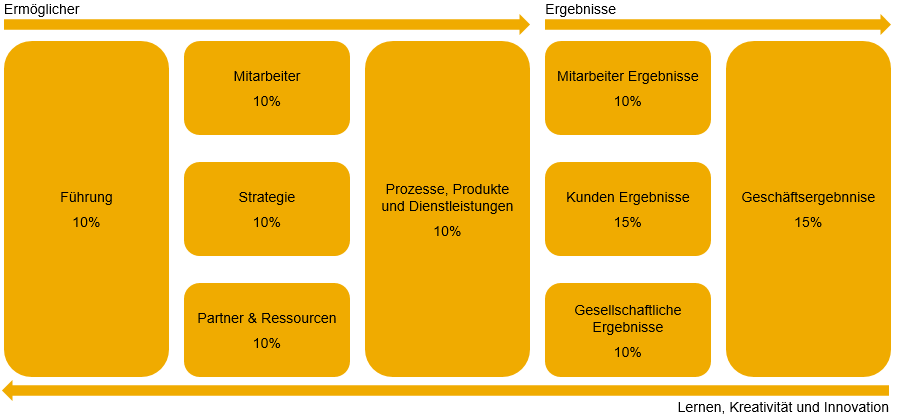
\includegraphics[width=\textwidth]{Abbildungen/efqmkat}
                    \caption[Kategorien zur Qualitätsbewertung von Unternehmen]{Kategorien zur Qualitätsbewertung von Unternehmen\protect\footnotemark}
                    \label{abb:efqm}
                \end{center}
            \end{figure}

            \footnotetext{Eigene Abbildung in Anlehnung an Pfitzinger (ISO 9000 zu TQM), S.30.}

            In \autoref{abb:efqm} werden die Kategorien der Bewertung von Qualität dargestellt. Die Ermöglicher auf der linken Seite nehmen dabei 50\% der möglichen Punkte ein, genau wie die Ergebnisse auf der rechten Seite. Die Ermöglicher bilden das Fundament der Qualität im Unternehmen und sind untereinander vernetzt. Hierbei geht eine umfassende Qualitätsstrategie von der Führung aus und muss von dieser gelebt werden. Von dort aus wird Spaltenweise gearbeitet. So werden die Mitarbeiter unter anderem von der Führung motiviert. Auch wird die Strategie zur Qualität von der Führung festgelegt.

            Nachdem der gesamte Prozess zwischen Ermöglichern und Ergebnissen durchlaufen und geprüft ist, kann die Führung auf Grundlage der Ergebnisse der Organisation nachjustieren und eine weitere Verbesserung anschließen. Somit beginnt ein Kreislauf, beziehungsweise eine kontinuierliche Verbesserung der Qualität.

            \subsubsection{Six Sigma}
            \label{subsec:sixsigma}

            Das Ziel Six Sigmas ist es \enquote{die Anforderungen des Kunden vollständig und profitabel [zu] erfüllen}\footnote{Knöfel (Six Sigma), S. 7}. Dabei ist neben dem externen Kunden, dem Abnehmer des Endprodukts, auch jeder interne Abnehmer eines Produktes gemeint. Sollte Abteilung B eines Unternehmens eine Fertigung von Abteilung A des gleichen Unternehmens weiterverarbeiten, so ist Abteilung B im Six Sigma Modell Kunde der Abteilung A. Auf diese Weise soll entlang der gesamten Prozesskette die Fehlerzahl gegen Null laufen.

            Six Sigma ist eine Methode, um möglichst perfekte Prozesse zu etablieren. Der Name dieser Methode entstammt der Statistik und entspricht der Zahl der Annahmequote von $6\sigma = 99.99966\%$. Dies bedeutet, dass beim Durchlauf von einer Millionen Prozessen, bzw. bei einer Millionen Endprodukte lediglich 3,4 Produkte fehlerhaft sind. Die Fehlerquote ist praktisch Null.\footnote{Vgl. Knöfel (Six Sigma), S.20f.}

            Um die Abweichungen zum Zielwert möglichst gering zu halten wird der Deming-Kreis, der im ISO 9001 Kapitel vorgestellt wurde, erweitert. Six Sigma verwendet den sogenannten DMAIC Verbesserungsprozess - Define, Measure, Analyse, Improve, Control - der aus dem Kaizen Prinzip entwickelt wurde. Der DMAIC Prozess wird durchlaufen, bis die Anforderungen des Kunden erfüllt wurden.\footnote{Vgl. Knöfel (Six Sigma), S.37ff.}

            \begin{figure}[!htbp]
                \begin{center}
                    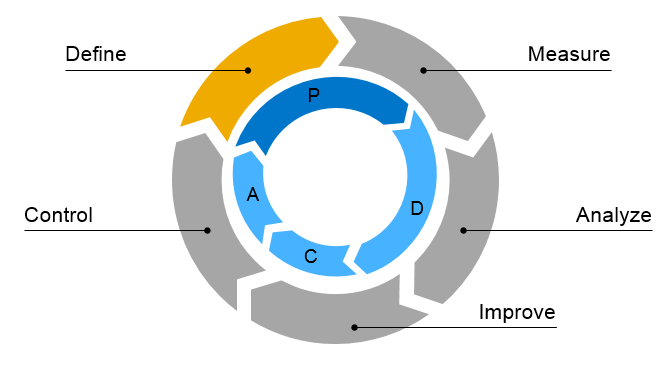
\includegraphics[width=11cm]{Abbildungen/pdcavsdmaic}
                    \caption{Kategorien zur Qualitätsbewertung von Unternehmen}
                    \label{abb:pdcavsdmaic}
                \end{center}
            \end{figure}

            In \autoref{abb:pdcavsdmaic} wird das Verhältnis des DMAIC Prozesses zum Deming-Kreis verbildlicht. In blau wird der Deming-Kreis mit den Phasen Plan, Do, Check und Act dargestellt, deren Anfangsbuchstaben in der Abbildung die jeweilige Phase markieren. Die Startpunkte der jeweiligen Zyklen sind jeweils farblich hervorgehoben.
            
            Im Folgenden werden die Phasen des DMAIC Prozesses vorgestellt und das jeweilige Äquivalent des Deming-Kreies erläutert.

            Zunächst wird die Problemstellung definiert. Das bedeutet, dass der Kunde befragt werden muss, welche Anforderungen er an den Prozess hat und welche Ausschuss- bzw. Fehlerrate er akzeptieren würde. Dies ist die Zielsetzung für den nachfolgenden Zyklus. Hierbei müssen die Kriterien messbar und binär, das heißt erfüllt oder nicht erfüllt, sein, damit in späteren Phasen geprüft werden kann, ob diese erfüllt sind.\footnote{Vgl. Knöfel (Six Sigma), S.42.} Die Definitionsphase des Prozesses stellt einen Teil der Planungsphase dar. Neben den Zielen wird auch die Vorgehensweise der nächsten Iteration geplant.

            Daraufhin wird das Maß festgelegt, an dem das Endergebnis gemessen wird. Die zuvor aufgenommenen Kundenanforderungen werden in statistische Messgrößen übersetzt und die zu messenden Kennzahlen festgelegt.
            Während eines Prozessdurchlaufs werden daraufhin Messdaten erfasst und gespeichert.\footnote{Vgl. Knöfel (Six Sigma), S.70.} Die Planungsphase erstreckt sich bis in die Messung hinein, da zu Beginn dieser Phase Verfahren zur Messung festgelegt werden. Die tatsächliche Messung findet im Rahmen der durchführenden (\emph{Do}) Phase statt und halten die Ergebnisse des durchlaufenen Prozesses fest.

            Die erfassten Daten werden nun analysiert und die Ursache der Abweichungen vom Zielwert wird erfasst.\footnote{Vgl. Knöfel (Six Sigma), S.124.} Die Analyse wird im Rahmen der \emph{Do} Phase durchgeführt und die Ergebnisse werden festgehalten, um der \emph{Improve} Phase als Grundlage zu dienen.

            Auf Grundlage dieser Abweichungen werden Verbesserungsvorschläge erarbeitet und der Mehrwert eben dieser wird beziffert. Zu beachten ist, dass die Ursache bekämpft werden soll und nicht die Symptome.\footnote{Vgl. Knöfel (Six Sigma), S.37.} Der bisherige Prozess wird geprüft (\emph{Check}), indem die Ergebnisse der Analyse mit den Wünschen der Planung und den vergangenen Iterationsergebnissen verglichen werden. Neben der Kontrolle, ob eine Verbesserung gegenüber früheren Iterationen vorliegt, können Möglichkeiten herausgearbeitet werden, um den Ablauf zu verbessern.

            Zuletzt werden Steuerungs- und Kontrollmöglichkeiten eingeführt, damit der verbesserte Prozess nachhaltig und konsistent umgesetzt wird. Das Six Sigma Team zieht sich zurück und überlässt die Kontrolle und den Prozess der ausführenden Abteilung.\footnote{Vgl. Knöfel (Six Sigma), S. 37.} Die Einführung dieser Verbesserungsmöglichkeiten und die Durchführung von Kontrollen deckt sich mit der \emph{Act} Phase des Deming-Kreises. 